\chapter*{}
\thispagestyle{empty}


\begin{center}
{\large\bfseries POSTCOVID-AI TelegramBot: facilitating data collection of people level human behavior }\\
\end{center}
\begin{center}
Juan del Río Gómez\\
\end{center}
\vspace{0.7cm}
\noindent{\textbf{Palabras clave}: chatbot, bienestar, inteligencia artificial, aplicación web}\\

\vspace{0.7cm}
\noindent{\textbf{Resumen}}\\

Este proyecto se centra en el desarrollo de un agente conversacional que permita la
recolección de datos relacionados con el bienestar de las personas. Forma parte del proyecto {\bfseries POSTCOVID-AI} como solución escalable a su método de recogida de datos mediante uso de otras tecnologías. El objetivo es facilitar esta recogida de datos para su posterior análisis a través de una herramienta que sea fácil de utilizar y atractiva a todo usuario.\vspace{0.3cm}

El chatbot guiará al usuario a través de preguntas específicas sobre su estado de ánimo,
actividades diarias, hábitos de sueño y alimentación entre otros aspectos. Además de recoger
datos, el bot dotará con herramientas de inteligencia artificial para ayudar al usuario a tomar
conciencia sobre el tema de conversación que estamos tratando.\vspace{0.3cm}

Gracias al procesamiento de lenguajes cada persona podrá hablar de forma escueta con el bot,
y a su vez este le irá haciendo una serie de preguntas previamente definidas. Todo esto se podrá definir y configurar a través de una aplicación web orientativa a la que el administrador tendrá acceso para poder
modificar las preguntas a realizar, agruparlas, añadir mensajes al bot y consultar los datos en tiempo real.


\cleardoublepage
\thispagestyle{empty}

\begin{center}
{\large\bfseries POSTCOVID-AI TelegramBot: facilitating data collection of people level human behavior }\\
\end{center}
\begin{center}
Juan del Río Gómez\\
\end{center}
\vspace{0.7cm}
\noindent{\textbf{keywords}: chatbot, well being, artificial intelligent, web application}\\

\vspace{0.7cm}
\noindent{\textbf{Abstract}}\\

This project focuses on the development of a conversational agent that allows for the collection of data
collection of data related to people's well-being. It is part of the {\bfseries POSTCOVID-AI} project as a scalable solution to its method of data collection using other technologies. The objective is to facilitate this data collection for subsequent analysis through a tool that is easy to use and attractive to all users.\vspace{0.3cm}

The chatbot will guide the user through specific questions about their mood, daily activities, sleeping and eating habits, among other aspects. In addition to collecting data, the bot will be equipped with artificial intelligence tools to help the user become aware of the topic of conversation we are dealing with.\vspace{0.3cm}

Thanks to language processing, each person will be able to speak briefly with the bot, and in turn, the bot will ask a series of previously defined questions. All this can be defined and configured through a web application to which the administrator will have access in order to be able to modify the questions to be asked, group them, add messages to the bot and consult the data in real time.

\chapter*{}
\thispagestyle{empty}

\noindent\rule[-1ex]{\textwidth}{2pt}\\[4.5ex]

Yo, \textbf{Juan del Río Gómez}, alumno de la titulación TITULACIÓN de la \textbf{Escuela Técnica Superior
de Ingenierías Informática y de Telecomunicación de la Universidad de Granada}, con DNI 46069380N, autorizo la ubicación de la siguiente copia de mi Trabajo Fin de Grado en la biblioteca del centro para que pueda ser consultada por las personas que lo deseen.

\vspace{5cm}

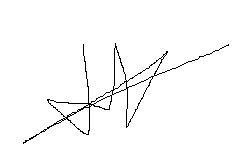
\includegraphics[width=0.4\textwidth]{imagenes/firma.png}\\[0.5cm]

\noindent Fdo: Juan del Río Gómez


\vspace{2cm}

\begin{flushright}
Granada a 1 de septiembre de 2023 .
\end{flushright}


\chapter*{}
\thispagestyle{empty}

\noindent\rule[-1ex]{\textwidth}{2pt}\\[4.5ex]

D. \textbf{Oresti Baños Legrán(tutor1)}, Profesor del Área de Ingeniería de Sistemas y Automática del Departamento de Ingeniería de Computadores, Automática y Robótica de la Universidad de Granada.

\vspace{0.5cm}

D. \textbf{Miguel Damas Hermoso (tutor2)}, Profesor del Área de de Ingeniería de Sistemas y Automática del Departamento de Ingeniería de Computadores, Automática y Robótica de la Universidad de Granada.


\vspace{0.5cm}

\textbf{Informan:}

\vspace{0.5cm}

Que el presente trabajo, titulado \textit{\textbf{POSTCOVID-AI TelegramBot}},
ha sido realizado bajo su supervisión por \textbf{Juan del Río Gómez (alumno)}, y autorizamos la defensa de dicho trabajo ante el tribunal
que corresponda.

\vspace{0.5cm}

Y para que conste, expiden y firman el presente informe en Granada a 1 de Septiembre de 2023.

\vspace{1cm}

\textbf{Los directores:}

\vspace{5cm}

\noindent \textbf{Oresti Baños Legrán (tutor1) \ \ \ \ \ Miguel Damas Hermoso(tutor2)}

\chapter*{Agradecimientos}
\thispagestyle{empty}

       \vspace{1cm}

En primer lugar quisiera agradecer a mi familia, sin su ayuda hoy no estaría donde estoy.

A todos mis compañeros de carrera y amigos, siempre dispuestos y atentos a ayudarme a resolver problemas del día a día.

Y a todos los profesores que me han aportado experiencias positivas gracias a su enseñanza durante el transcurso de esta bonita etapa. 
    


